\documentclass[a4paper,12pt,openany]{book}
\usepackage[utf8]{inputenc}
\usepackage{a4wide}
\usepackage{graphicx}
\usepackage{listings}
\usepackage{amsmath}
\usepackage{booktabs}
\usepackage[top=3cm, bottom=2cm, left=3cm, right=2cm]{geometry}
\lstset{language=Python, basicstyle=\ttfamily\small, frame=single, breaklines=true, literate={á}{{\'a}}1 {ã}{{\~a}}1 {é}{{\'e}}1 {°C}{{\textdegree C}}1 {ç}{{\c{c}}}1 {í}{{\'i}}1 {ó}{{\'o}}1 {ú}{{\'u}}1}

\title{Fundamentos de Machine Learning para Iniciantes}
\author{Ronald A. Mendonça}
\date{2025}

\begin{document}

\maketitle{}
\tableofcontents{}

\newpage

\section{Introdução}
Machine Learning (ML), ou aprendizado de máquina, é uma área da inteligência artificial que permite que sistemas computacionais 
identifiquem padrões e façam previsões a partir de dados, sem a necessidade de programação explícita para cada tarefa. Diferente de 
softwares tradicionais, onde regras são definidas manualmente, em ML os algoritmos aprendem diretamente com exemplos, ajustando-se 
para melhorar seu desempenho ao longo do tempo. Essa capacidade transformou campos como medicina, finanças e tecnologia, tornando-se 
uma das competências mais valiosas do século XXI.

A relevância do Machine Learning está em sua aplicabilidade prática. Empresas utilizam ML para prever vendas, detectar fraudes e 
personalizar recomendações, enquanto cientistas o aplicam para analisar dados complexos, como sequências genéticas ou padrões climáticos. 
Para o iniciante, entender os fundamentos de ML abre portas para uma carreira em ciência de dados ou simplesmente para compreender melhor
o mundo movido a dados em que vivemos.

Este eBook é voltado para iniciantes que desejam dar os primeiros passos em Machine Learning, sem experiência prévia na área. Para facilidade de 
entendimento, é recomendável um conhecimento básico de matemática (como médias e equações lineares) e familiaridade mínima com programação, 
preferencialmente em Python, embora os conceitos sejam explicados de forma acessível. Nosso objetivo é desmistificar o ML, oferecendo 
uma base teórica para quem quer iniciar a construir modelos simples e entender seus resultados.

Ao longo das próximas páginas, você será introduzido aos conceitos essenciais de Machine Learning, desde a manipulação de dados até a criação 
de modelos de regressão, classificação e clustering. Cada capítulo combina teoria com exemplos práticos, incluindo trechos de código em 
Python para ilustrar a aplicação dos métodos discutidos. Ao final, você terá conteúdo suficiente para construir um modelo de machine learning 
simples e entender os princípios que o sustentam.

\chapter{Conceitos Fundamentais: Dados e Aprendizado}

\section{Dados}
Em um determinado dia no seu trabalho, você se depara com o desafio de extrair respostas de um conjunto de infromações que, a príncipio, não parecem fazer
muito sentido para você. Estruturados ou não, podem ser números, textos, imagens ou qualquer outro tipo de informação. Isso é o que chamamos de dados.
Os dados são a base de qualquer modelo de Machine Learning. São coletados, organizados e analisados para extrair informações valiosas.

\begin{itemize}
    \item \textbf{Dados Qualitativos (ou Categóricos):} Representam características ou atributos que não podem ser quantificados numericamente.
    \begin{itemize}
        \item \textbf{Nominais:} Não possuem ordem natural. Ex: cores (vermelho, azul, verde), tipos de frutas.
        \item \textbf{Ordinais:} Possuem uma ordem ou hierarquia. Ex: níveis de satisfação (ruim, regular, bom, ótimo), ranking de qualidade (A, B, C).
    \end{itemize}

    \item \textbf{Dados Quantitativos (ou Numéricos):} Representam valores numéricos e podem ser medidos.
    \begin{itemize}
        \item \textbf{Discretos:} Assumem valores inteiros e finitos. Ex: número de filhos, número de carros em um estacionamento.
        \item \textbf{Contínuos:} Podem assumir qualquer valor dentro de um intervalo. Ex: altura, peso, temperatura.
    \end{itemize}
\end{itemize}

\section{Importância da Compreensão dos Tipos de Dados}
Entender os tipos de dados é essencial para escolher os algoritmos adequados e preparar os dados corretamente. 
Dados quantitativos podem ser usados diretamente em modelos numéricos, enquanto qualitativos e textuais requerem pré-processamento. Essa distinção será 
explorada em detalhes nos capítulos seguintes, onde veremos como transformar e utilizar esses dados em tarefas práticas de Machine Learning.


\section{Tipos de Aprendizado}
Os tipos de aprendizado de máquina podem ser classificados em três categorias principais: 
Supervisionado, Não Supervisionado e Aprendizado por Reforço.

\subsection{Aprendizado Supervisionado (Supervised Learning)}
O aprendizado supervisionado ocorre quando o modelo é treinado em um conjunto de dados rotulado, ou seja, onde a saída correta é 
conhecida. O objetivo do modelo é aprender um mapeamento entre as entradas e as saídas corretas.
    \begin{itemize}
        \item Previsão de preços de imóveis
        \item Diagnóstico médico
        \item Classificação de e-mails como spam ou não spam
    \end{itemize}


\subsection{Aprendizado não Supervisionado (Unsupervised Learning)}
No tipo de aprendizado não supervisionado, os dados não são rotulados e o modelo deve identificar padrões e estruturas nos dados de forma autônoma.
    \begin{itemize}
        \item Segmentação de clientes
        \item Compressão de dados
        \item Detecção de anomalias
    \end{itemize}

\subsection{Aprendizado por Reforço (Reinforcement Learning)}
O aprendizado por reforço se baseia em um agente que aprende interagindo com um ambiente e recebendo recompensas ou penalidades com base em suas ações.
\begin{itemize}
    \item Jogos e Inteligência Artificial (xAI, OpenAI, DeepSeek)
    \item Controle de robôs
\end{itemize}

\begin{table}[ht]
    \centering
    \begin{tabular}{p{4cm} p{6cm} p{4cm}}
    \toprule
    \textbf{Aprendizado} & \textbf{Descrição} & \textbf{Tipo de Dados} \\ 
    \midrule
    Supervisionado & Dados rotulados & Qualitativos e Quantitativos\\
    Não Supervisionado & Usa dados não rotulados para encontrar padrões & Quantitativos \\
    Por Reforço & Aprendizado por tentativa e erro, com recompensas & Qualitativos e Quantitativos \\ 
    \bottomrule
    \end{tabular}
    \caption{Comparação entre os tipos de aprendizado de máquina e os tipos de dados utilizados.}
    \label{tab:tipos_aprendizado}
    \end{table}



\chapter{Estatística Essencial para Machine Learning}  

\section{Estatística Descritiva}
A estatística descritiva é uma parte fundamental da análise de dados, pois fornece uma visão geral das características principais de um conjunto de dados.
Ela envolve o resumo e a descrição dos dados por meio de medidas numéricas, gráficos e tabelas. As principais medidas incluem:
\begin{itemize}
    \item \textbf{Média:} A média aritmética é a soma de todos os valores dividida pelo número total de valores.
    \item \textbf{Mediana:} O valor que separa os dados em duas metades, onde 50\% dos dados estão abaixo e 50\% estão acima.
    \item \textbf{Moda:} O valor que aparece com mais frequência em um conjunto de dados.
    \item \textbf{Variância:} Uma medida da dispersão dos dados em relação à média. A variância é calculada como a média dos quadrados das diferenças entre cada valor e a média.
    \item \textbf{Desvio Padrão:} Uma medida da dispersão dos dados em relação à média. Quanto maior o desvio padrão, mais espalhados estão os dados.
    \item \textbf{Correlação:} Uma medida que indica a força e a direção da relação entre duas variáveis. A correlação varia de -1 a 1, onde -1 indica uma correlação negativa perfeita, 0 indica nenhuma correlação e 1 indica uma correlação positiva perfeita.
\end{itemize}

\subsection{Exemplo: Calculando a Média e o Desvio Padrão de Temperaturas Diárias}

Suponha que registramos as temperaturas máximas diárias (°C) de uma semana em uma cidade. Os dados coletados são: 20, 22, 19, 23, 21, 20, 24. Vamos calcular a média e o desvio padrão passo a passo.

\subsubsection{Cálculo da Média}
A média (\(\bar{x}\)) é obtida somando todos os valores e dividindo pelo número de observações (\(n\)). Matematicamente:
\begin{equation}
\bar{x} = \frac{\sum_{i=1}^{n} x_i}{n}
\end{equation}
Para os dados fornecidos:
\begin{itemize}
    \item Soma dos valores: \(20 + 22 + 19 + 23 + 21 + 20 + 24 = 149\),
    \item Número de observações: \(n = 7\),
    \item Média: \(\bar{x} = \frac{149}{7} \approx 21.29\).
\end{itemize}
Portanto, a temperatura média diária é aproximadamente 21,29°C.

\subsubsection{Cálculo do Desvio Padrão}
O desvio padrão (\(\sigma\)) mede a variabilidade dos dados em relação à média. Para uma população, é dado por:
\begin{equation}
\sigma = \sqrt{\frac{\sum_{i=1}^{n} (x_i - \bar{x})^2}{n}}
\end{equation}
Passo a passo:
\begin{enumerate}
    \item Calcule as diferenças entre cada valor e a média (\(x_i - \bar{x}\)):
    \begin{itemize}
        \item \(20 - 21.29 = -1.29\),
        \item \(22 - 21.29 = 0.71\),
        \item \(19 - 21.29 = -2.29\),
        \item \(23 - 21.29 = 1.71\),
        \item \(21 - 21.29 = -0.29\),
        \item \(20 - 21.29 = -1.29\),
        \item \(24 - 21.29 = 2.71\).
    \end{itemize}
    \item Eleve cada diferença ao quadrado:
    \begin{itemize}
        \item \((-1.29)^2 = 1.6641\),
        \item \(0.71^2 = 0.5041\),
        \item \((-2.29)^2 = 5.2441\),
        \item \(1.71^2 = 2.9241\),
        \item \((-0.29)^2 = 0.0841\),
        \item \((-1.29)^2 = 1.6641\),
        \item \(2.71^2 = 7.3441\).
    \end{itemize}
    \item Some os quadrados: \(1.6641 + 0.5041 + 5.2441 + 2.9241 + 0.0841 + 1.6641 + 7.3441 = 19.4288\),
    \item Divida pelo número de observações: \(\frac{19.4288}{7} \approx 2.7755\),
    \item Tire a raiz quadrada: \(\sigma = \sqrt{2.7755} \approx 1.66\).
\end{enumerate}
Assim, o desvio padrão das temperaturas é aproximadamente 1,66°C.

\subsubsection{Interpretação}
A média de 21,29°C indica a temperatura típica da semana, enquanto o desvio padrão de 1,66°C mostra que as temperaturas variam, em média, 1,66°C para mais ou menos em relação à média. Esses valores ajudam a entender a consistência do clima e podem ser usados em modelos de Machine Learning para previsões futuras.

\subsubsection{Cálculo com Python}
Os mesmos cálculos podem ser realizados de forma eficiente usando Python com a biblioteca NumPy. O código a seguir mostra como:

\begin{lstlisting}[language=Python]
# Importando a biblioteca NumPy
import numpy as np
    
# Dados das temperaturas diárias
temperaturas = [20, 22, 19, 23, 21, 20, 24]
    
# Calcula a média
media = np.mean(temperaturas)
print(f"Média das temperaturas: {media:.2f}°C")
    
# Calcula o desvio padrão
desvio_padrao = np.std(temperaturas)
print(f"Desvio padrão das temperaturas: {desvio_padrao:.2f}°C")
\end{lstlisting}    

Executando o código, obtemos uma média de 21,29°C e um desvio padrão de 1,67°C, valores consistentes com o cálculo manual (pequenas diferenças ocorrem devido a 
arredondamentos).
    
\subsubsection{Visualização com Curva Normal}
A distribuição das temperaturas pode ser visualizada em uma curva normal, que mostra como os dados se distribuem em torno da média. A Figura~\ref{fig:curva_normal} apresenta o histograma das temperaturas e a curva normal correspondente, gerada com Python e as bibliotecas Matplotlib e SciPy.
    
\begin{figure}[ht]
\centering
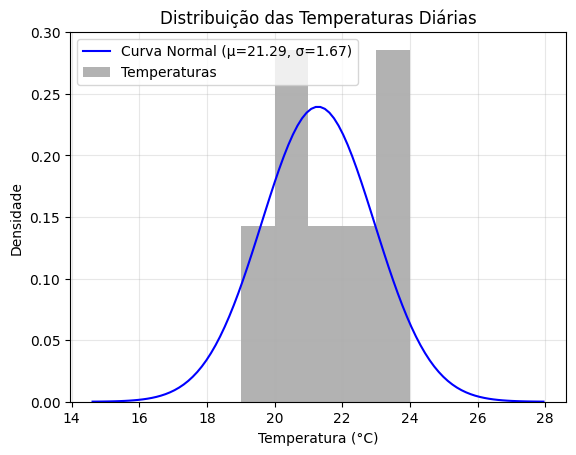
\includegraphics[width=0.8\textwidth]{curva_normal_temperaturas.png}
\caption{Distribuição das temperaturas diárias com curva normal (média = 21,29°C, desvio padrão = 1,67°C).}
\label{fig:curva_normal}
\end{figure}
    
\subsubsection{Interpretação}
A média de 21,29°C e o desvio padrão de 1,67°C indicam que as temperaturas variam moderadamente em torno de um valor central. A curva normal na Figura~\ref{fig:curva_normal} ilustra essa distribuição, sendo útil em Machine Learning para entender a variabilidade dos dados antes de aplicar modelos preditivos.

\end{document}  



